

% \section{}

\subsection{Thesis}%{This work}

{

\newcommandx{\uthev}[2][1=1-]{\textbf{\textcolor<#1>{B2}{#2}}}
\newcommandx{\gifarge}[2][1=1-]{\textcolor<#1>{B2}{#2}}
\begin{frame}[c]{\gifarge[2]{Spacetime ripples} from \gifarge[3]{domain-wall wiggles}}


    % \note<1>{In medias res..\par Would not recommend playing the drining game or whatever that says you have to drink every time I say ``but we will not discuss this here''\dots}

    % \medskip
    % \only<1>{\textbf{ANNA:}
    % \begin{enumerate}
    %     \item Animasjoner---satt av noe tid i helgen
    %     \item Leselighet (PP)
    %     \item Hva kan sløyfes?
    % \end{enumerate}
    % }
    % \only<1>{\textcolor{DUMMY1}{Drinking game: one shot for every time I say ``but we will not discuss this here''\dots }}
    
    \uncover<2->{Gravitational waves (GWs) are \uthev[2]{ripples} travelling through \uthev[2]{spacetime} at the speed of light, generated by the acceleration of massive objects. }
    % \note[item]<2>{... giving rise to the particle interpretation; the hypothesised massless spin-2 boson called gravitational}
    % \note[item]<2>{As EM waves, they are characterised by a frequency and different instruments are needed to observe different frequency ranges, and different ranges give different physical insight.} 

    % \only<2>{\textcolor{uiogrey}{\small%
    % In the high- and intermediate-frequency ranges\footnote[2]{$\sim 10^{[-5,4]} \unit{Hz}$; detected with space- and Earth-based interferometers}, GWs are typically sourced by \emph{astrophysical sources}, e.g.~black-hole binaries.}}
    % \note[item]<2>{Circular motion = acceleration}
    \ifOnlyNotes\else
    \only<2>{
        \begin{textblock*}{0.5\paperwidth}(0.5\paperwidth, 0.26\paperheight)
            \begin{flushright}
                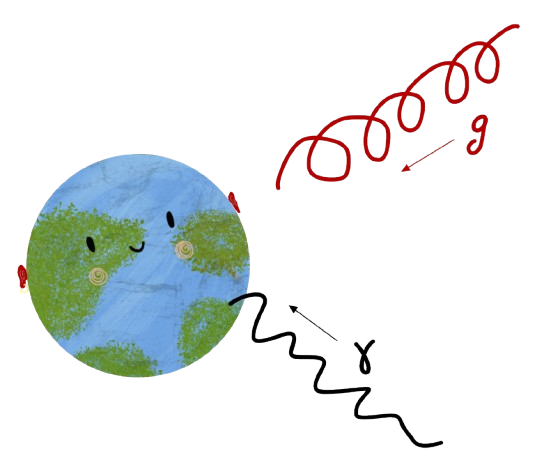
\includegraphics[height=0.72\paperheight,keepaspectratio]{figs/GW_EM_Earth.png}
            \end{flushright}
        \end{textblock*}
    }\fi
 
    
    \uncover<3->{\medskip
        Potential sources of low-frequency GWs 
        %\only<3>{\footnote[3]{$\lesssim 10^{-7}\unit{Hz}$; detected with e.g.~Pulsar Timing Arrays (PTAs)}}
        are topological defects, such as spatially perturbed---\uthev[3]{<<wiggly>>}---\uthev[3]{domain walls} (DWs). 
    % \comment{Consider figure.}
    }

    % \only<3>{\textcolor{uiogrey}{\small%
    % Cosmological defects are generally relics of phase transitions, which themselves can produce gravitational radiation.}}

    % \note[item]<3>{As part of a stochastic gravitational wave background}
    % \note[item]<3>{Wavelengths in order of years}
    % \note[item]<3>{Walls separating two vacua.}


    \uncover<4->{\medskip
        \small\gifarge[4]{\paragraph{Main aim.}}%
        Gain \emph{analytical} insight to the dynamics of cosmic DWs in conformally flat Friedmann--Lema\circumflex{i}tre--Robertson--Walker (FLRW) spacetime, to search for its GW footprint.
        % \[
        % \text{Aims:}\begin{cases}
        %     \text{}
        % \end{cases}
        % \]
        \only<5>{
            \ifOnlyNotes\else
            \begin{textblock*}{\textwidth}(1cm, 0.78\paperheight)
                \textcolor{R1}{\textbf{But why?}}
            \end{textblock*}
            \fi
        }   

    }


% *************************************
% NOTES *******************************
\begin{notes}[5][title \& aim]
    \nnote{1}{In medias res; first about the thesis, title, aims, motivation}
    \itnote{2}{\small
        \item particle interp.; hypothesised massless spin-2 boson \newconcept{graviton}
        \item Like EM waves, observations in different frequency bands require different instruments and carry  different information  insight to the universe -> two different ``sensory impressions''
        \item On Earth, we have been able to see for a long time, but we \textcolor{O1}{developed hearing in 2015}
        % \item If EM waves are the Earth's eyes, GWs are the ears; observations of these waves give a new type of insight (sensory impression) 
        % \item developed hearing in 2015
        % \item As EM waves; characterised by a frequency, and different instruments are needed to observe different frequency ranges, and different ranges give different physical insight\dots
        \item high-freq: BH binaries \textcolor{G1}{[hand gesture]}
    }
    \itnote{3}{
        \item \textcolor{O1}{colliding, collapsing or otherwise interacting/imperfect}
        \item generally relics of PTs, which themselves can produce GW rad.
    }
    \itnote{4}{
        \item topological defects in context of a first-order late-time (redshift around 2, matter domination) PT
    }
\end{notes}
% *************************************
\end{frame}
}



% \begin{frame}{Motivation}
%     \uncover<1->{\paragraph{Aims.}%
%     {%
%     Study the dynamics of topological defects in a generic spacetime. Specifically,
%     gain analytical insight to DW dynamics in expanding spacetime, in order to study its GW footprint. Test the applicability of the thin-wall approximation.}}
%     %

%     \medskip
%     \only<2>{\textcolor{R1}{\textbf{But why?}}}

%     % \begin{description}[font=\scshape]
%     %     \item[\descItem{relevance}]<3-> 
%     %     \only<4->{\scriptsize}{Recent PTA-observations\only<3>{\citef{agazieNANOGrav15Yr2023}} provide evidence for a stochastic GW background (GWB) in cosmological frequency ranges.}%
%     %     \note<5>{* Astrophysical sources cannot explain the GW signal >> new physics?}
%     %     \item[\descItem{demand}]<4-> 
%     %     \only<5->{\scriptsize}{Close the knowledge gap between ranges \textcolor{DUMMY1}{help}}
%     %     \item[\descItem{applicability}]<5-> 
%     %     \only<6->{\scriptsize}{Substitution to computationally expensive simulations. }
%     %     \item[\descItem{convenience}]<6-> 
%     %     \only<7->{\scriptsize}{DWs are intuitive structures \textcolor{DUMMY1}{help}}
%     % \end{description}

    
%     % \only<7>{
%     %     \medskip
%     %     \textcolor{O1}{\textbf{But are we successful?}}}
    

% \end{frame}


% \begin{frame}{\unfinishedSlide~Aims}
%     \comment{FIXME}
%     \begin{itemize} 
%         \item Gain analytical insight 
%         \item Study the dynamics of topological defects in a generic spacetime.
%         \item Specifically, gain analytical insight to DW dynamics when the metric is Friedmann--Lema\circumflex{i}tre--Robertson--Walker (FLRW), in order to study its GW footprint. 
%         \item Test the applicability of the thin-wall approximation.
%     \end{itemize}

%     \medskip
%     \uncover<2>{\textcolor{R1}{\textbf{But why?}}}


% % *************************************
% % NOTES *******************************
% \begin{notes}[2][aims]
%     \nnote{1}{jeodf}
% \end{notes}
% % *************************************
% \end{frame}




\begin{frame}{Motivation}

    % \bigskip

    
    \begin{description}[font=\scshape]
        % \note<1>{\textit{Why cosmological GWs?}\par}
        % ---------
        % RELEVANCE
        \item[\descItem{relevance}]<1-> 
        \textcolor<2->{uiogrey}{Recent observations\invisible<2->{\footnote<1>{\cite{agazieNANOGrav15Yr2023}}} %
        % \only<1>{\citef{agazieNANOGrav15Yr2023}} 
        provide evidence for a stochastic GW background (GWB) in cosmological frequency ranges. Future GW experiments aim at similar frequency ranges.}%
        %
        % \note<1>{* Astrophysical sources cannot explain the GW signal >> new physics?\par}
        % \note<1>{* \comment{EXAMPLES}\par}
        % \note<1>{\noteNext{\textit{Why theoretical and analytical focus?}} }
        % ------
        % DEMAND
        \item[\descItem{demand}]<2-> 
        \textcolor<3->{uiogrey}{Analytical estimates allow possibly arbitrary dynamical ranges; ranges inaccessible in cosmological simulations.}%{Close the knowledge gap between ranges \textcolor{DUMMY1}{help}}
        %
        % \note<2>{* Lack of analytical solutions in generic spacetimes?\par}
        % \note<2>{\noteNext{(same) \textit{Why theoretical and analytical focus?}}}
        % -----------
        % CONVENIENCE
        \item[\descItem{convenience}]<3-> 
        \textcolor<4->{uiogrey}{Substitution to computationally expensive relativistic simulations.}
        % 
        % \note<3>{\noteNext{\textit{Why topological defects?}}}
        % -------------
        % APPLICABILITY
        \item[\descItem{applicability}]<4->
        \textcolor<5->{uiogrey}{Topological defects are ubiquitous in physics.} 
        % 
        % \note<4>{\noteNext{\textit{Why domain walls?}}}
        % ----------
        % SIMPLICITY
        \item[\descItem{simplicity}]<5->
        \textcolor<6->{uiogrey}{DWs are good pedagogies for topological defects.}
        % 
        % \note<5>{* Intuitive structures}
    \end{description}

    % \note<6>{\noteNext{With this in mind, let us back up a bit}}

    
% *************************************
% NOTES *******************************
\begin{notes}[6][motivation]
    \nnote{1}{\textit{Why interest in cosmological GWs?} {---Astrophysical sources cannot explain the GW signal >> new physics?}}
    \nnote{2}{\textit{Why theoretical and analytical focus?} {---Lack of analytical solutions in generic spacetimes?}}
    \nnote{3}{\textit{(same)}}
    \nnote{4}{\textit{Why topological defects?}}
    \nnote{5}{\textit{Why domain walls?} {---Intuitive structures}}
    \nnote{6}{With this in mind, let us back up a bit}
\end{notes}
% *************************************

\end{frame}



% |||||||||||||||||||||
% ||||| Overview ||||||
% |||||||||||||||||||||




% \subsection{Overview}





% \begin{frame}{Overview of project \comment{remove?}}
%     We will\comment{blah blah}
%     {
%     % \newcommand{\boldLastStep}[1]{\only{\textbf{#1}}<4>}

%     % \newcommand{\fld}{\textsc}% field
%     \newcommand{\ths}{\textcolor{uioblue1}} % we will cover

%     \begin{description}[font=\scshape]
%         \item[\descItem{classical field theory} ]<1-> {perturbation theory}, {action principles}, \only{\ths}<4>{topological defects}
%         \item[\descItem{differential geometry} ]<2-> {pseudo-Riemannian manifolds}, conformal transformations, \only{\ths}<4>{hypersurfaces}%, tensor perturbations
%         \item[\descItem{modern cosmology} ]<3-> {concordance model}, \only{\ths}<4>{gravitational waves}
%     \end{description}
%     }
% \end{frame}


% \begin{frame}[plain]%{Project overview}
%     \begin{textblock*}{0.98\paperwidth}(0.2cm,0.6cm)
%         \foreach \x in {1,...,7}{
%                 \only<\x>{\adjincludegraphics%
%                 [width=0.98\paperwidth,trim={{0.08\width} {0.4\height} {0.08\width} {0.1\height}},clip]%
%                 {figs/Page\x.png}}
%         }%
%     \end{textblock*}
%     % \uiobigimage{?}
% \end{frame}


% \uiobigimage{Overview}


